\newpage
\appendix
\setcounter{figure}{0} %図番号のリセット
\section{付録}
\subsection{外皮作成方法}
本研究において,外皮は先行研究\cite{kyu}を参考に作製したが,型の準備手順を一部変更したので以下に記す.
\begin{enumerate}
    \item 型やシリコンと振れる面に離型剤(GSIクレオス社,VM008)を塗る.これは,外皮が完成した際にシリコンが型や中子からはがれやすくするために使用する.
    \item 離型剤が乾いたら型で中子を挟む.この時,先行研究\cite{kyu}ではゴムシートを挟んでシリコンが漏れ出ないようにしていたが,本研究では図\ref{fig:atugami}のような厚紙(大創産業社製,工作用紙)を使用した.
    \item 型を板で挟み,板ごと万力で固定したら型の準備は完了.
\end{enumerate}

\subsection{作製した基板}
本研究で作製した基板について述べる.本基板は基板CAD「EAGLE」で設計を行い,基板加工機(LPLF ProtMat S43)を使用して作製した.駆動部と制御部は電気的に絶縁し,フォトカプラ(Isocom Components製,TLP621-2)
を用いて制御信号をモータ側に伝えている.図\ref{fig:kiban}に設計した基板を,図\ref{fig:kiban_kousei}に回路のブロック図を示す.
\begin{figure}[hb]
    \centering
    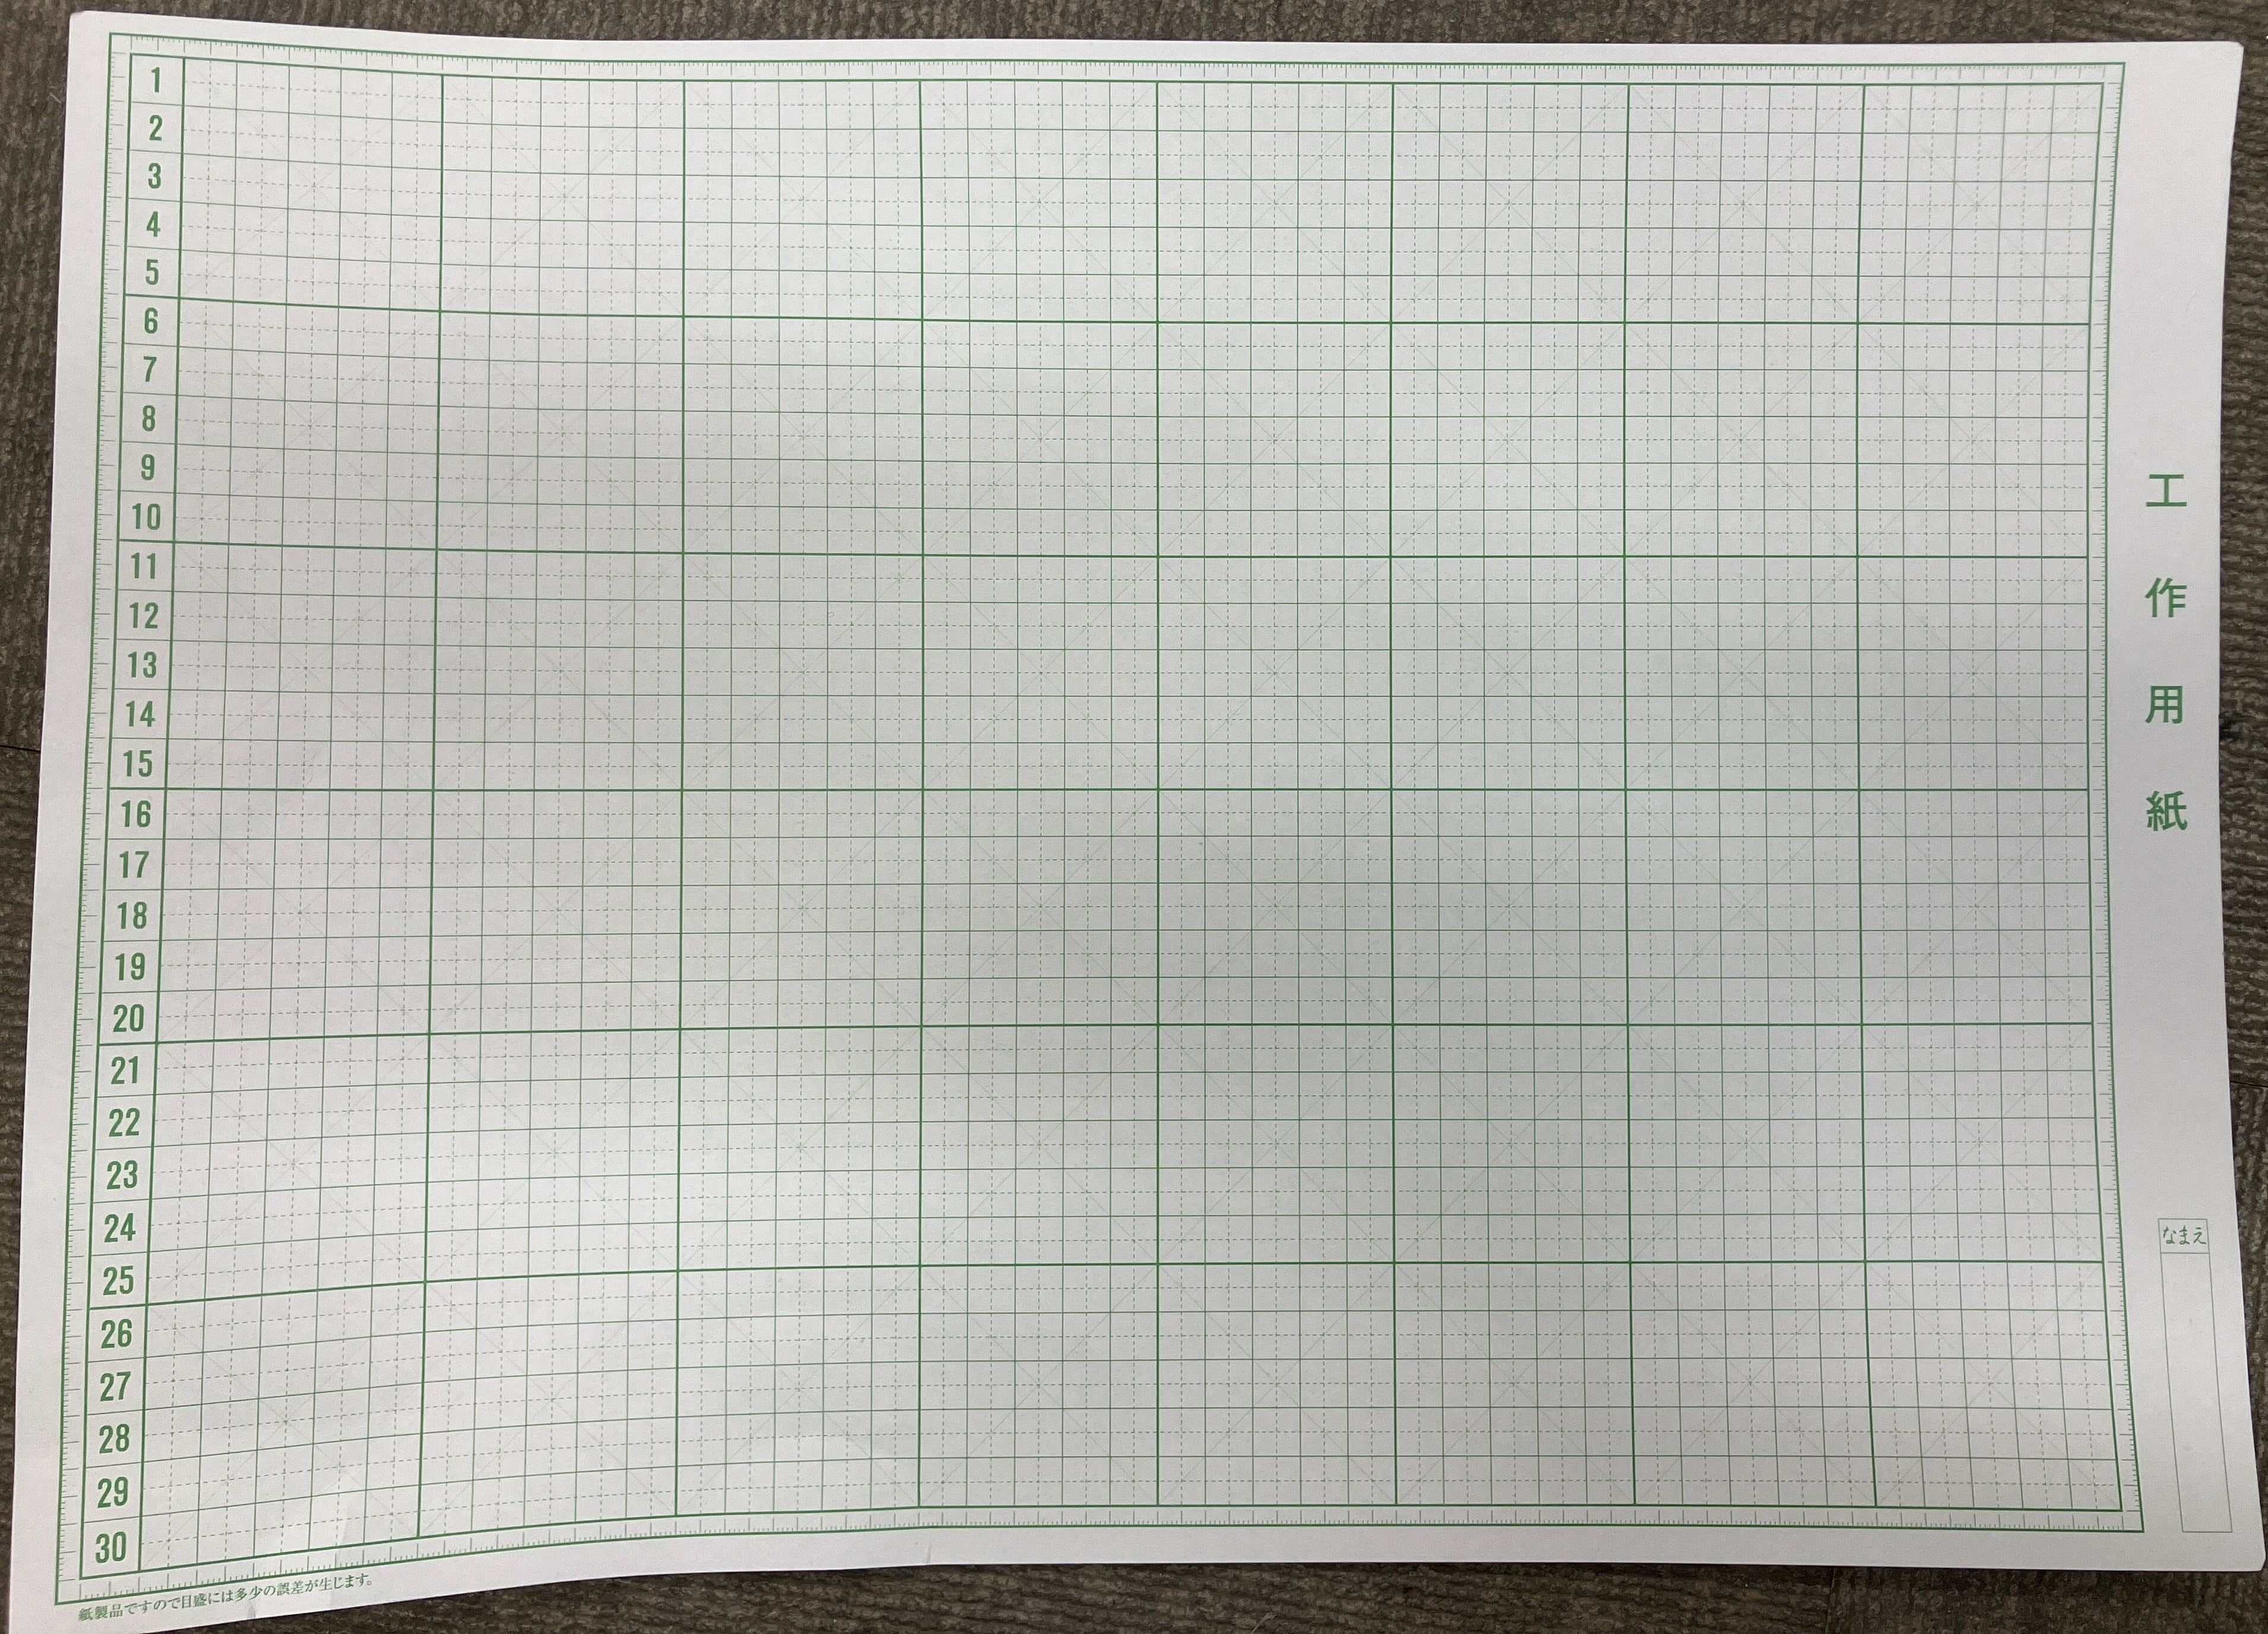
\includegraphics[width=0.6\linewidth]{chapters/picture/atugami.jpg}
    \caption{使用した厚紙}
    \label{fig:atugami}
\end{figure}
\begin{figure}[t]
    \centering
    \begin{tabular}{cc}
        \begin{minipage}[b]{0.4\linewidth}
            \centering
            \setPicture{kiban.png}
            \subcaption{設計した基板}
            \label{fig:kiban_cad}
        \end{minipage}
        \hspace{0.1\linewidth}
        \begin{minipage}[b]{0.4\linewidth}
            \centering
            \setPicture{kiban_real.jpg}
            \subcaption{実際の写真}
            \label{fig:kiban_real}
        \end{minipage}
    \end{tabular}
    \caption{作製した基板}
    \label{fig:kiban}
\end{figure}
\begin{figure}[t]
    \centering
    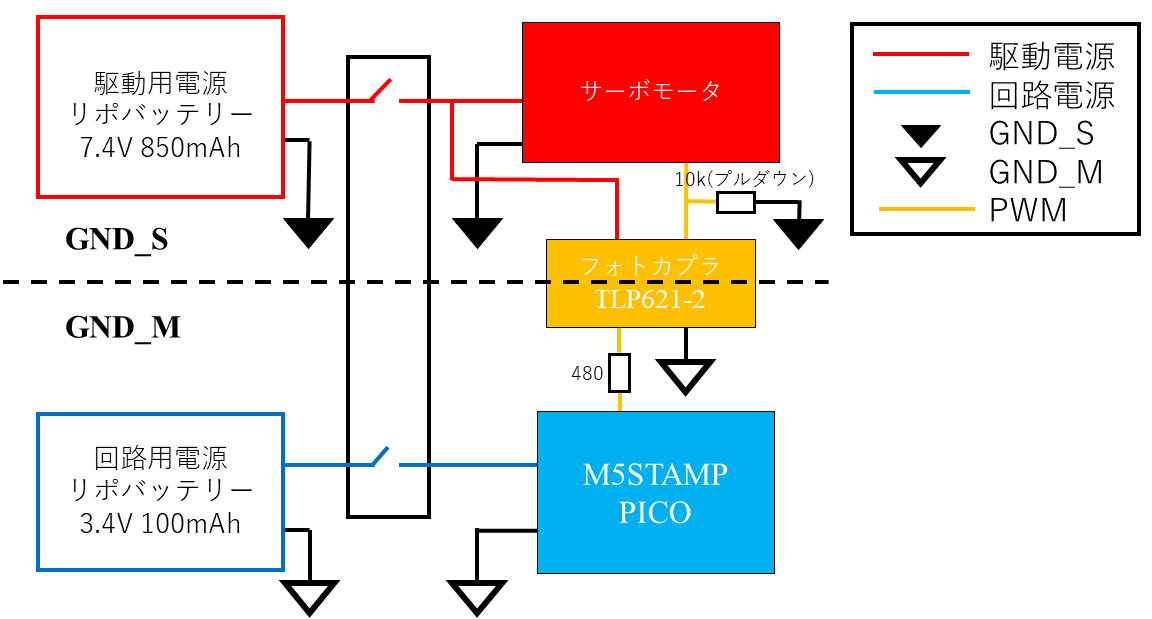
\includegraphics[width=0.9\linewidth]{chapters/picture/kiban_kousei.png}
    \caption{基板の構成}
    \label{fig:kiban_kousei}
\end{figure}
